\section{Introduction}
\begin{frame}[fragile]
  \frametitle{ADTs}

  An Algrebraic Data Type is a composite type made of other types

  \begin{example}
    \begin{lstlisting}
      type List[A]   = Nil | Cons[A]
      type Option[A] = None | Some[A]


      sealed trait Tree
      case class Name() extends Tree
      case class Select(qual: Tree, name: Name) extends Tree
      case class Method(fun: Tree, args: ArgClauses) extends Tree
      case class If(p: Tree, thenp: Tree, elsep: Tree) extends Tree

      case class ArgClauses(args: List[List[Tree]]) extends Tree
    \end{lstlisting}
  \end{example}
\end{frame}

\begin{frame}
  \frametitle{Failure handling}

  \begin{table}[h]
    \centering
    \begin{tabular}{cccccc}
      \toprule
       &                 & \textbf{Null}s & \textbf{Exception}s & \textbf{ADT}s & \\
      \midrule
       & Difficulty      & Easy           & Easy                & Less easy     & \\
       & Failure reason  & Unknown        & Known               & Known         & \\
       & Performances    & Best           & Bad                 & Better        & \\
       & Expressivity    & Bad            & Better              & Best          & \\
       & Runtime failure & Possible       & Possible            & No            & \\
    \end{tabular}
  \end{table}

  \begin{table}[h]
    \centering
    \begin{tabular}{rcccc}
      \textbf{Benchmark}   & \textbf{Mode} & \textbf{Count} & \textbf{Score} & \textbf{Error} \\
      \midrule
      No exceptions        & avgt          & 10             & 0.046          & ± 0.003        \\
      Throw \& catch       & avgt          & 10             & 16.268         & ± 0.239        \\
      Throw \& no catch    & avgt          & 10             & 17.874         & ± 3.199        \\
      Throw w/o stacktrace & avgt          & 10             & 1.174          & ± 0.014        \\
      \bottomrule
    \end{tabular}
    \caption{Comparison \& Benchmarks (ms/op)}
  \end{table}
\end{frame}

\begin{frame}[fragile]
  \frametitle{Parser combinators}

  Create a complex parser from simple ones

  \begin{example}
    \begin{lstlisting}
      val tpeSep: Parser[String]  // ( : ) | (: ) | ( :)
      val alphas: Parser[Char]    // [a-zA-Z]
      val name: Parser[String]    = alphas.repeat.combineAll

      // Parser[Param] -- x: Int
      (name <* tpeSep).product(name).map(???)

      // Parser[Queue[Param]] -- // x: A, y: B, z: C
      (paramParser <* paramSepParser).repeat
        .combineWith(Queue.empty)(_ :+ _)
        .product(paramParser.orElse(Parser.empty))
        .map(???)
    \end{lstlisting}
  \end{example}
\end{frame}

\begin{frame}[fragile]
  \frametitle{Parser combinators --- example}

  \begin{overprint}
    \onslide<1>
    Given the following code, which parser can we create?
    \begin{example}
      \begin{lstlisting}
        package scalala
  
        object Main:
          val x = 1
          val y = 2
          val adder = (a: Int, b: Int) => a + b
  
          def main(args: Array[String]): Unit =
            println(foo(x, y))
  
          def foo(x: Int, y: Int) = x + y
      \end{lstlisting}
    \end{example}

    \onslide<2>
    \begin{table}
      \centering
      \begin{tabular}{rll}
        \toprule
        \textbf{Parser}    & \textbf{Description}  & \textbf{Example}                                    \\
        \midrule
        \texttt{name}      & A simple name         & \texttt{x}, \texttt{y}, \texttt{main}, \texttt{foo} \\
        \texttt{literal}   & A literal value       & \texttt{1}, \texttt{2}                              \\
        \texttt{val}       & A value definition    & \texttt{val x = 1}                                  \\
        \texttt{param}     & A method parameter    & \texttt{a:Int}, \texttt{args:Array[String]}         \\
        \texttt{paramList} & A parameter list      & \texttt{a:Int, b:Int}                               \\
        \texttt{method}    & A method definition   & \texttt{main(args:Array[String]) = }                \\
        \texttt{function}  & A function definition & \texttt{adder = (a:Int, b:Int) => }                 \\
        \texttt{class}     & A class definition    & \texttt{object Main}                                \\
        \texttt{source}    & A source file         & \texttt{package scalala; ...}                       \\
        \bottomrule
      \end{tabular}
    \end{table}

    \onslide<3>
    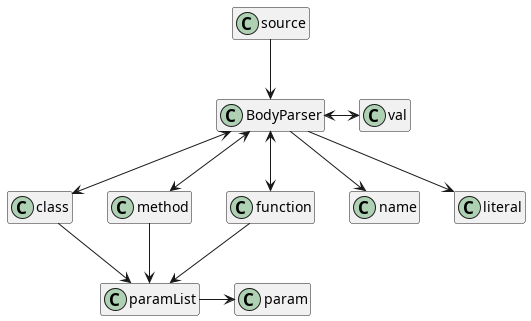
\includegraphics[width=0.96\textwidth]{img/parser-structure.png}
  \end{overprint}
\end{frame}

\begin{frame}[fragile]
  \frametitle{General approach}

  \begin{overprint}
    \onslide<1>
    With \(\mathcal{P}\) the parser algrebra and \(\mathcal{A}\) the ADT algebra. I'll use reification to implement this parser, with 3 kinds of methods:
    \begin{itemize}
      \item Constructors \(c\): \(\forall x \notin \mathcal{P}, c(x) \in \mathcal{P}\)
      \item Combinators \(f\): \(\forall c_1, c_2 \in \mathcal{P}, f(c_1, c_2) \in \mathcal{P}\)
      \item Interpreters \(z\): \(\forall c \in \mathcal{P}, x \notin \mathcal{P}, z(c, x) \in \mathcal{A}\)
    \end{itemize}
  
    \begin{example}[Reification methods]
      \begin{lstlisting}[gobble=8]
        // Constructor
        def string(s: String): Parser[String]
        // Combinator
        def orElse[A, B](p1: Parser[A], p2: Parser[B]): Parser[A | B]
        // Interpreter
        Parser[A].parse(input: String): A
      \end{lstlisting}
    \end{example}
    
    \onslide<2>
    For each abstract concept, we'll have a concrete implementation (with a \texttt{case class}) and reification methods. For instance, for a simple string parser and a simple mapper:
    
    \begin{lstlisting}
      trait Parser[+A]:
        def map[B](f: A => B): Parser[B] = ParserMap(this, f)
      object Parser:
        def string(s: String): Parser[String] = ParserString(s)
    
      case class ParserString(s: String) extends Parser[String]
      case class ParserMap[A, B](
        source: Parser[A],
        f: A => B
      ) extends Parser[B]
    \end{lstlisting}
  \end{overprint}
\end{frame}
